\documentclass[12pt]{beamer}
\usepackage[english]{babel}
\usepackage[utf8]{inputenc}
\usepackage[T1]{fontenc}
\usepackage{lmodern}
\usepackage{minted}
\usepackage{graphicx}

\makeatletter

\setbeamersize{text margin left=1em,text margin right=1em}

\setbeamerfont{title}{series=\bfseries,size=\LARGE}
\setbeamerfont{subtitle}{series=\bfseries,size=\Large}
\setbeamerfont{frametitle}{series=\bfseries,size=\small}
\setbeamerfont{block title}{series=\bfseries,size=\normalsize}
\setbeamerfont{footline}{size=\normalsize}

\usebeamercolor{structure}
\setbeamercolor{normal text}{fg=structure.fg}

\addtobeamertemplate{frametitle}{}{\vspace*{-1ex}\rule{\textwidth}{1pt}}

\setbeamertemplate{itemize items}[circle]

\setbeamertemplate{navigation symbols}{}

\setbeamertemplate{footline}{
   \centering
   \begin{minipage}{\dimexpr\paperwidth-\beamer@leftmargin-\beamer@rightmargin\relax}
   \centering
   \rule{\linewidth}{1pt}\vskip2pt
   \usebeamerfont{footline}
   \usebeamercolor{footline}
   \hfill\insertframenumber/\inserttotalframenumber
   \hfill
   \llap{\insertframenavigationsymbol\insertbackfindforwardnavigationsymbol}\par
   \end{minipage}\vskip2pt
}

\makeatother

\newcommand{\mycomment}[1]{}

\graphicspath{ {./img/} }

\title{Automation of chlorination in a water treatment plant}
\author{Arena M., Corriera F., Orlando T.}
\institute{Università degli studi di Messina}
\date{05/07/2023}

\begin{document}

\begin{frame}
\maketitle
\end{frame}

\begin{frame}
\frametitle{Summary}
\begin{itemize}
\item General idea
\item Functional Requirements
\item Tables
\item Sequential Function Chart
\item Ladder Diagram
\item Components choice
\end{itemize}
\end{frame}

\begin{frame}
\frametitle{General Idea}
\framesubtitle{}
A water treatment plant is designed to remove impurities and contaminants from raw water sources to produce safe and clean drinking water. The treatment process typically consists of several stages, including:
\begin{itemize}
    \item Pre-treatment
    \item Coagulation and Flocculation
    \item Sedimentation
    \item Filtration
    \item Disinfection or Chlorination
    \item Final testing and Distribution
\end{itemize}
\end{frame}

\begin{frame}
\frametitle{General Idea}
\framesubtitle{Chlorination stage}
Chlorination is a process of adding chlorine to water to kill harmful microorganisms, such as bacteria, viruses, and protozoans, that can cause waterborne illnesses. Chlorine is a powerful disinfectant and is widely used in water treatment plants around the world.
\end{frame}

\begin{frame}
\frametitle{General Idea}
\framesubtitle{Chlorination steps}
The chlorination process typically involves the following steps:
\begin{enumerate}
    \item Pre-chlorination
    \item Primary chlorination
    \item Chlorine contact time
    \item Dechlorination
\end{enumerate}
\end{frame}

\begin{frame}
\frametitle{Functional Requirements}
\framesubtitle{}
Assuming that the pre-chlorination process is regulated in another infrastructure by another PLC, we isolate our case of study to the management of just the chlorination tank.
\end{frame}

\begin{frame}
\frametitle{Functional Requirements}
\framesubtitle{}
\begin{itemize}
    \item Manage the water intake, checking the water levels in the tank
    \item Manage the chlorine emission, checking the chlorine concentration
    \item Mix the water with the chlorine
    \item Let the water rest for 30 minutes
    \item Manage the chlorated water outgo
    \item Be able to manage problematic scenarios
    \item Be able to stop the process
    \item Be able to resume the process
    \item Manage two different outputs of water:
    \begin{itemize}
        \item Normal outtake to procede with the water treatment process
        \item Drain to free the tank of unusable water
    \end{itemize}
\end{itemize}
\end{frame}

\begin{frame}
\begin{figure}
    \centering
    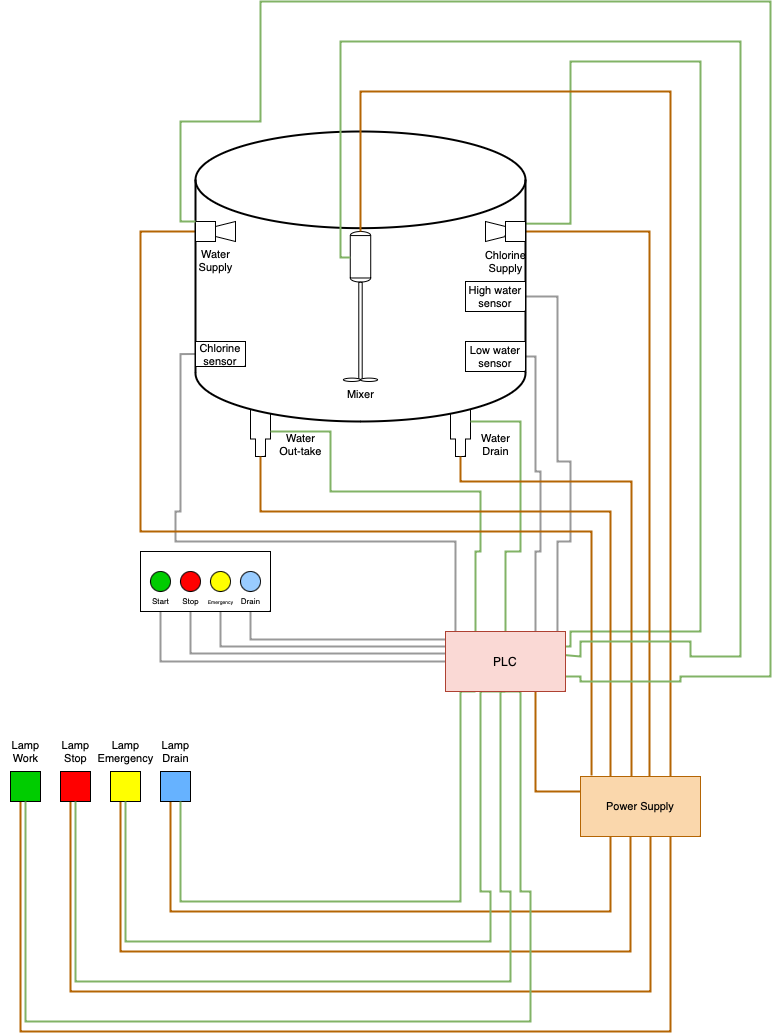
\includegraphics[trim={0 0 0 0}, clip, scale=.22]{img/Tank_draw.png}
    \label{fig:tank_draw}
\end{figure}
\end{frame}

\begin{frame}
\frametitle{Tables}
\framesubtitle{Inputs}
\begin{table}[]
    \centering
    \begin{tabular}{|c|c|c|}
        \hline
        Label & I/O Address & Comment \\
        \hline
        \hline
        Start & I0.0 & Start button\\
        \hline
        WL1 & I0.1 & Low water level sensor\\
        \hline
        WL2 & I0.2 & High water level sensor\\
        \hline
        CH1 & I0.3 & Residual chlorine sensor\\
        \hline
        Stop & I0.4 & Stop button\\
        \hline
        Drain & I0.5 & Drain button\\
        \hline
        Emergeny & I0.6 & Emergency stop button\\
        \hline
    \end{tabular}
    \caption{Input table}
    \label{tab:inputs}
\end{table}
\end{frame}

\begin{frame}
\frametitle{Tables}
\framesubtitle{Outputs}
\begin{table}[]
    \centering
    \begin{tabular}{|c|c|c|}
    \hline
       Label & I/O Address & Comment \\
       \hline
       \hline
       HL1 & Q0.0 & Lamp work\\
       \hline
       HL2 & Q0.1 & Lamp stop\\
       \hline
       HL3 & Q0.2 & Lamp emergency stop\\
       \hline
       HL4 & Q0.3 & Lamp emergency drain\\
       \hline
       PM1 & Q0.4 & Pump for water intake\\
       \hline
       PM2 & Q0.5 & Pump for water drain\\
       \hline
       PM3 & Q0.6 & Pump for emergency drain\\
       \hline
       PM4 & Q0.7 & Pump for chlorine supply\\
       \hline
       M1 & Q1.0 & Mixer\\
       \hline
    \end{tabular}
    \caption{Output table}
    \label{tab:outputs}
\end{table}
\end{frame}

\begin{frame}
\frametitle{Tables}
\framesubtitle{Internal Variables}
\begin{table}[]
    \centering
    \begin{tabular}{|c|c|c|}
    \hline
       Label & I/O Address & Comment\\
       \hline
       \hline
       State0 & M2.0 & SFC state variable\\
       \hline
       State1 & M2.1 & ''\\
       \hline
       State2 & M2.2 & ''\\
       \hline
       State3 & M2.3 & ''\\
       \hline
       State4 & M2.4 & ''\\
       \hline
       State5 & M2.5 & ''\\
       \hline
       State6 & M2.6 & ''\\
       \hline
       State7 & M2.7 & ''\\
       \hline
       SS & MB0 & Suspended state value\\
       \hline
    \end{tabular}
    \caption{Internal varibles table}
    \label{tab:internal_variables}
\end{table}
\end{frame}

\begin{frame}
\frametitle{Sequential Function Chart}
\framesubtitle{}
\begin{figure}
    \centering
    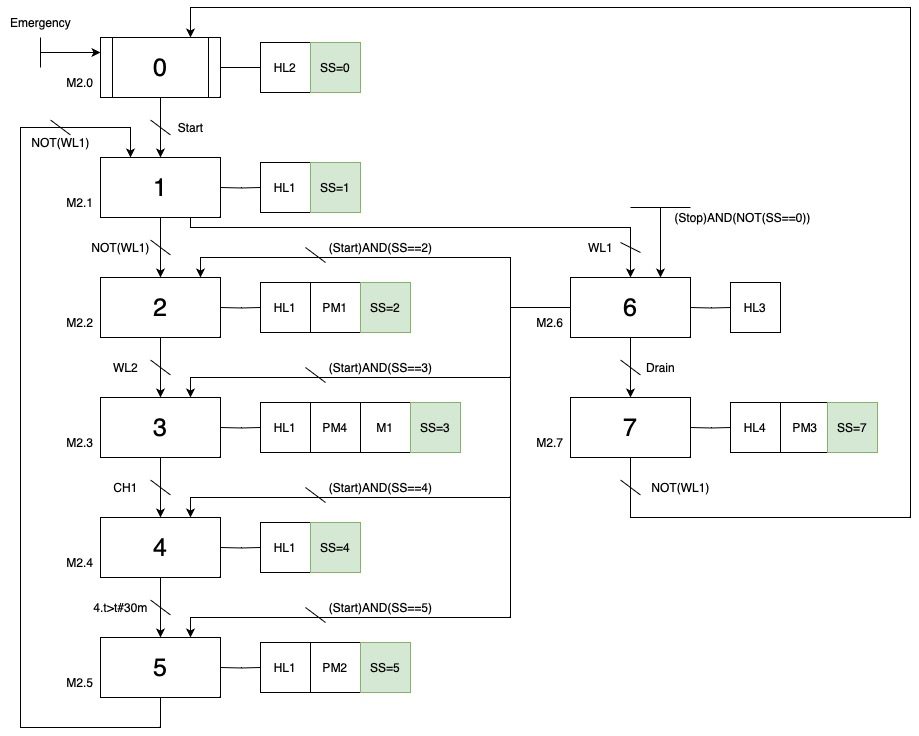
\includegraphics[scale=.24]{img/SFC.jpg}
    \caption{SFC Diagram}
    \label{fig:sfc}
\end{figure}
\end{frame}

\begin{frame}
\frametitle{Ladder Diagram}
\framesubtitle{Initialization}
\begin{figure}
    \centering
    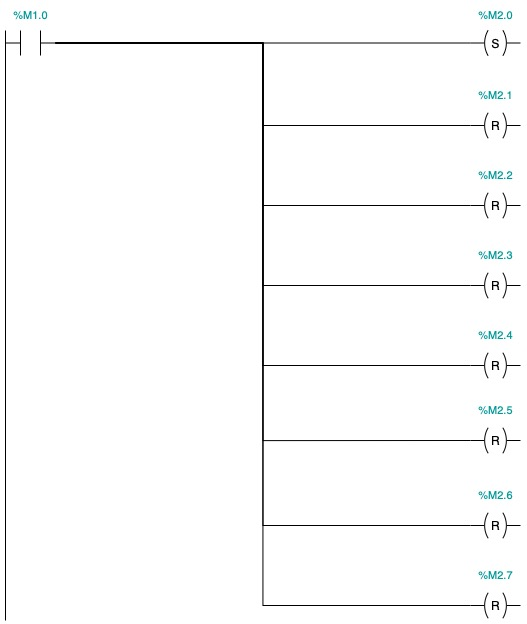
\includegraphics[trim={0 11cm 0 0}, clip, scale=.5]{img/Ladder_diagram_1.jpg}
    \caption{Initialization - Ladder diagram part 1}
    \label{fig:ladder11}
\end{figure}
\end{frame}

\begin{frame}
\frametitle{Ladder Diagram}
\framesubtitle{Initialization}
\begin{figure}
    \centering
    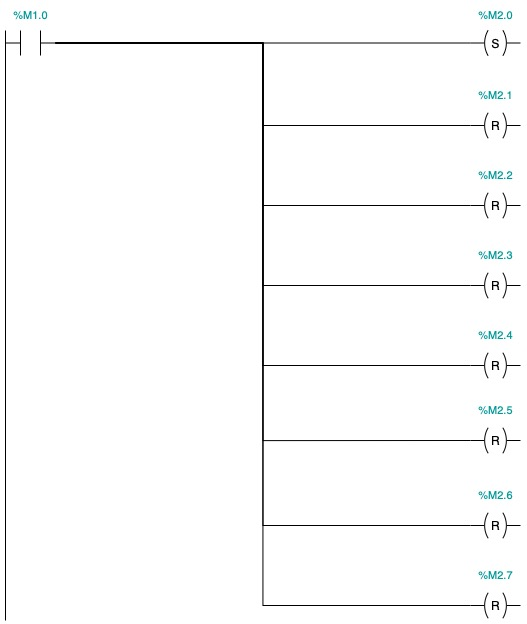
\includegraphics[trim={0 0 0 11cm}, clip, scale=.5]{img/Ladder_diagram_1.jpg}
    \caption{Initialization - Ladder diagram part 2}
    \label{fig:ladder12}
\end{figure}
\end{frame}

\begin{frame}
\frametitle{Ladder Diagram}
\framesubtitle{State Machine}
\begin{figure}
    \centering
    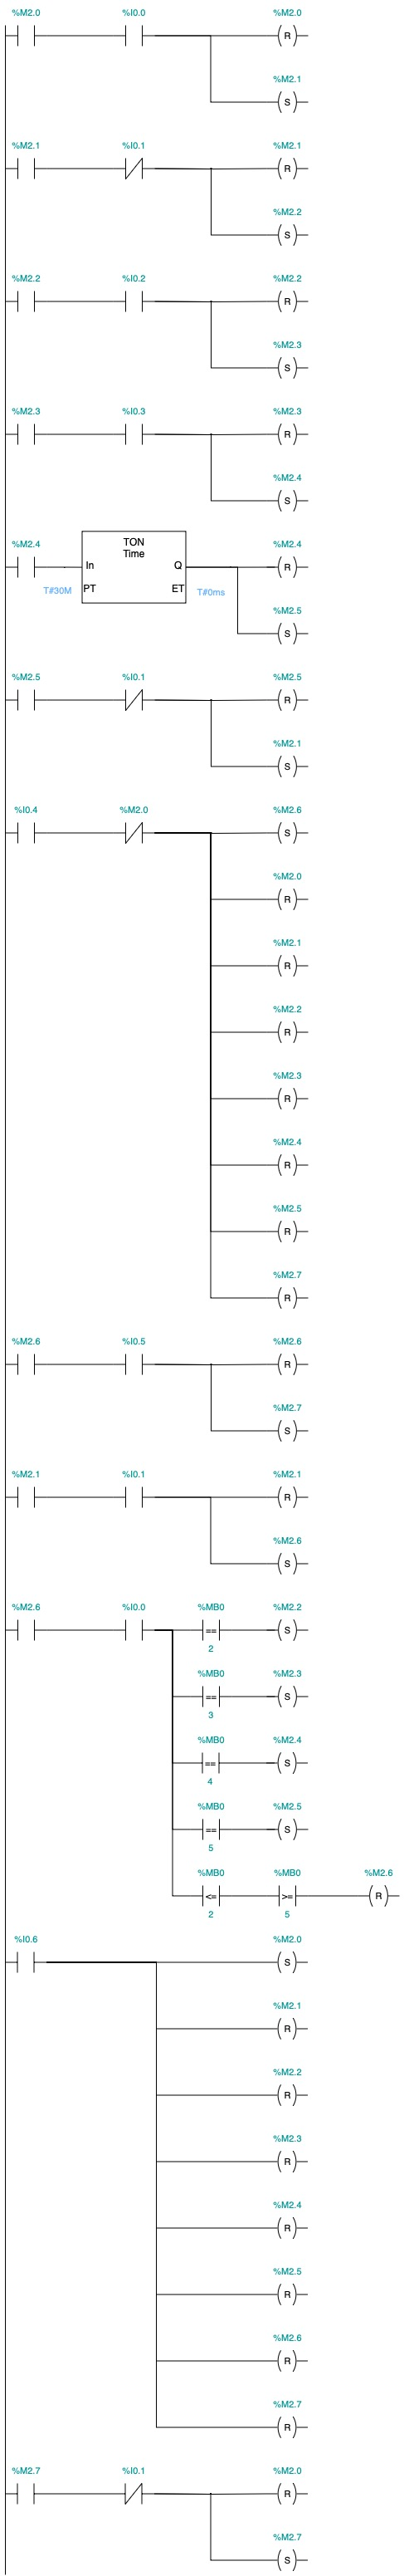
\includegraphics[trim={0 98cm 0 0}, clip, scale=.5]{img/Ladder_diagram_2.jpg}
    \caption{State Machine - Ladder diagram part 1}
    \label{fig:ladder21}
\end{figure}
\end{frame}

\begin{frame}
\frametitle{Ladder Diagram}
\framesubtitle{State Machine}
\begin{figure}
    \centering
    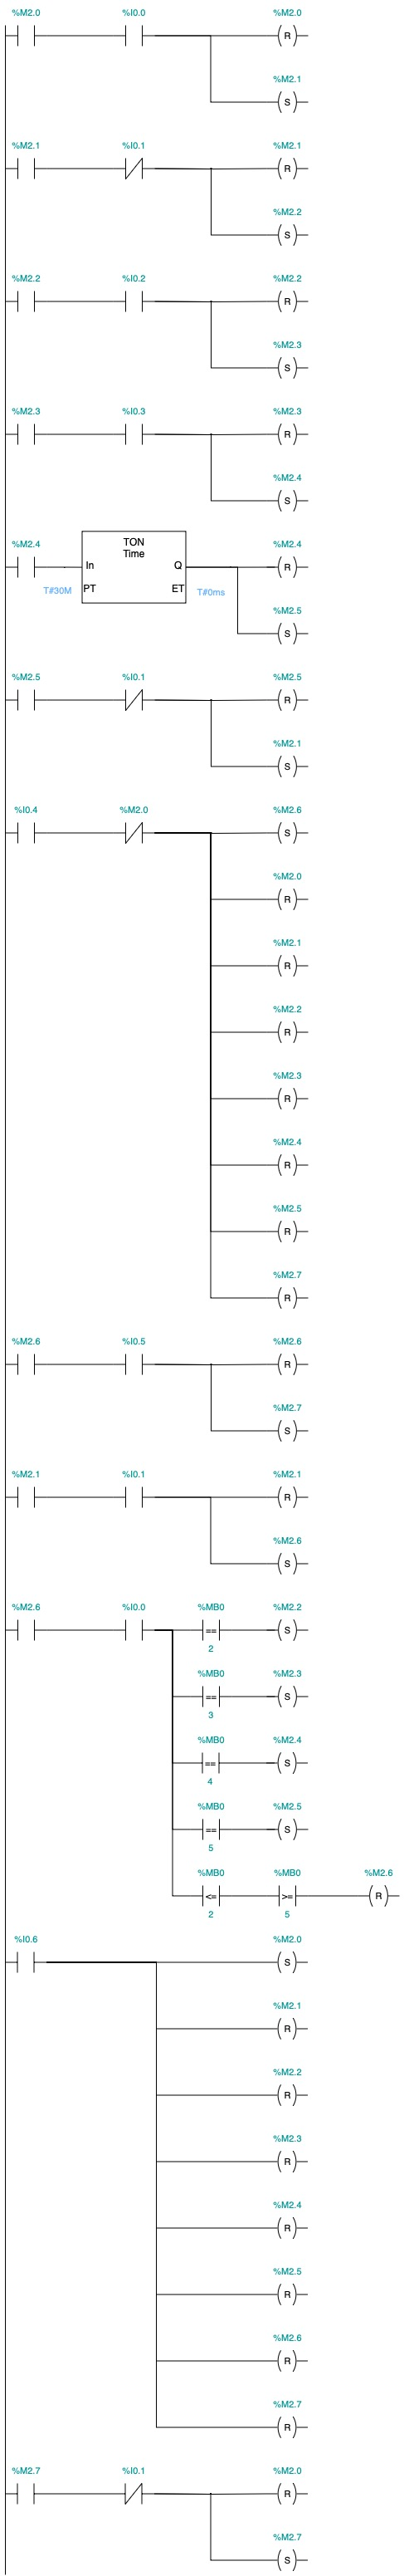
\includegraphics[trim={0 87cm 0 11cm}, clip, scale=.5]{img/Ladder_diagram_2.jpg}
    \caption{State Machine - Ladder diagram part 2}
    \label{fig:ladder22}
\end{figure}
\end{frame}

\begin{frame}
\frametitle{Ladder Diagram}
\framesubtitle{State Machine}
\begin{figure}
    \centering
    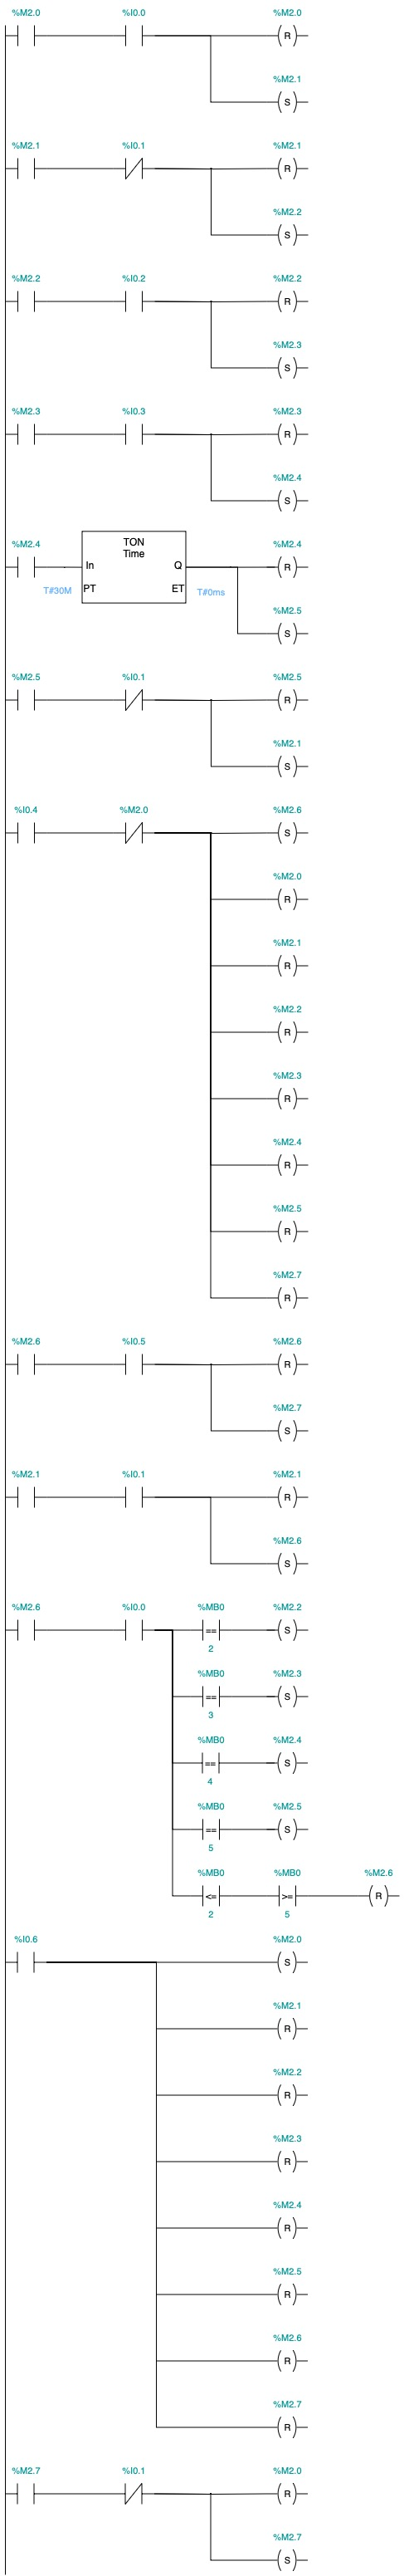
\includegraphics[trim={0 76cm 0 22cm}, clip, scale=.5]{img/Ladder_diagram_2.jpg}
    \caption{State Machine - Ladder diagram part 3}
    \label{fig:ladder23}
\end{figure}
\end{frame}

\begin{frame}
\frametitle{Ladder Diagram}
\framesubtitle{State Machine}
\begin{figure}
    \centering
    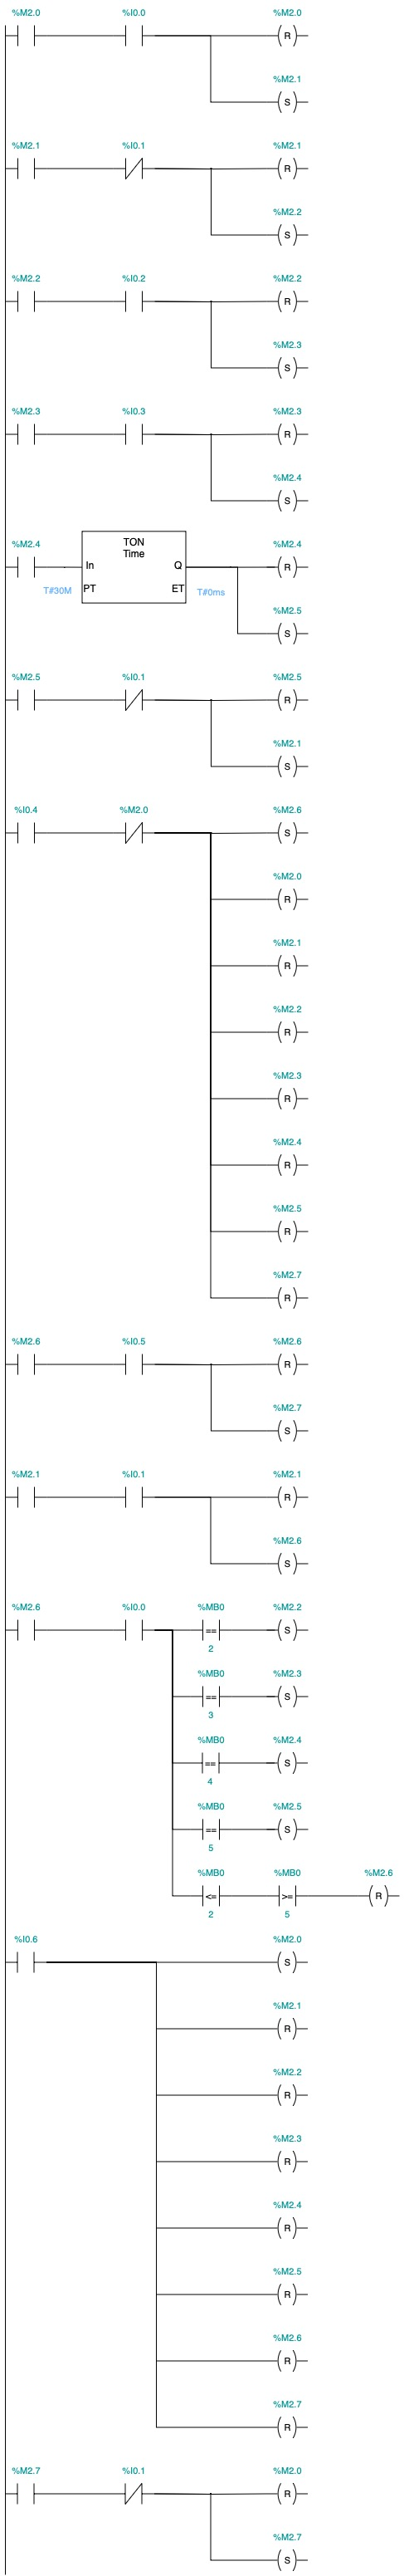
\includegraphics[trim={0 65cm 0 33cm}, clip, scale=.5]{img/Ladder_diagram_2.jpg}
    \caption{State Machine - Ladder diagram part 4}
    \label{fig:ladder24}
\end{figure}
\end{frame}

\begin{frame}
\frametitle{Ladder Diagram}
\framesubtitle{State Machine}
\begin{figure}
    \centering
    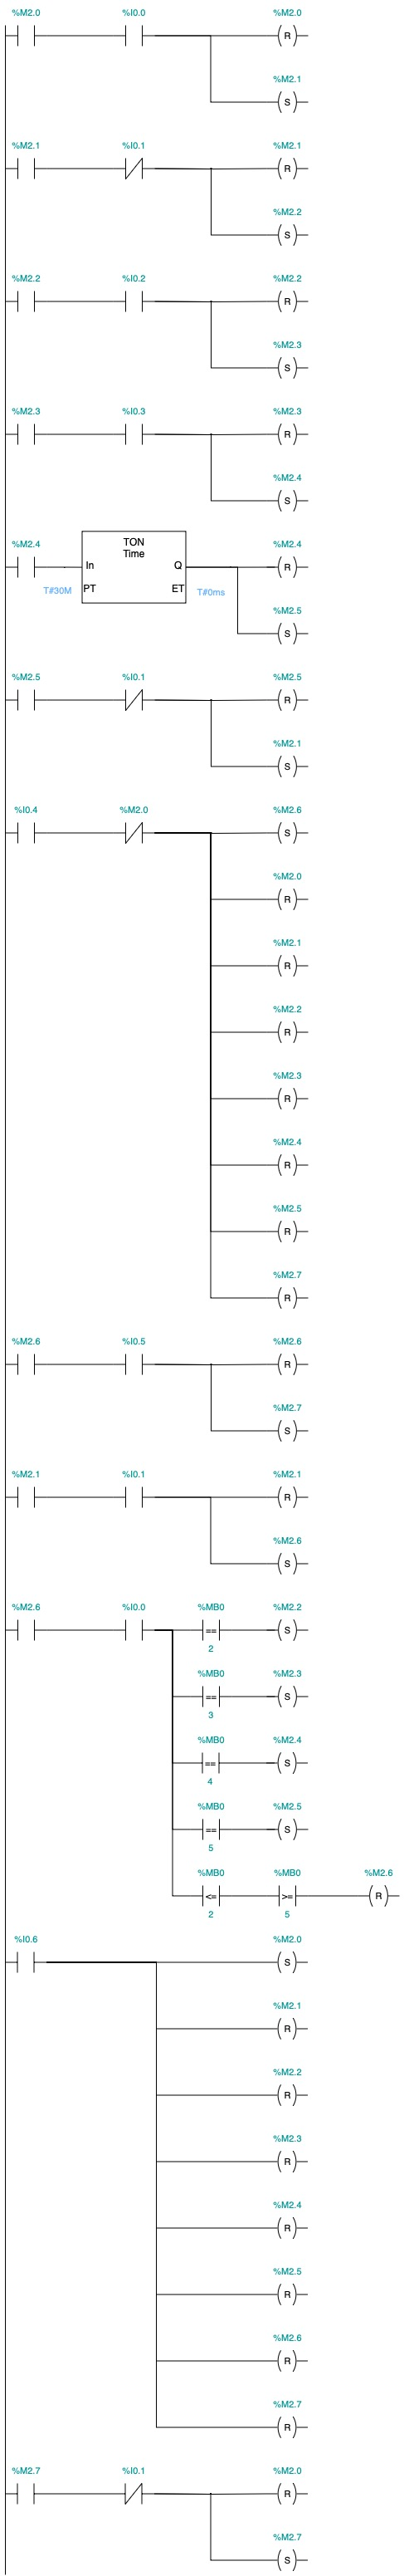
\includegraphics[trim={0 54cm 0 44cm}, clip, scale=.5]{img/Ladder_diagram_2.jpg}
    \caption{State Machine - Ladder diagram part 5}
    \label{fig:ladder25}
\end{figure}
\end{frame}

\begin{frame}
\frametitle{Ladder Diagram}
\framesubtitle{State Machine}
\begin{figure}
    \centering
    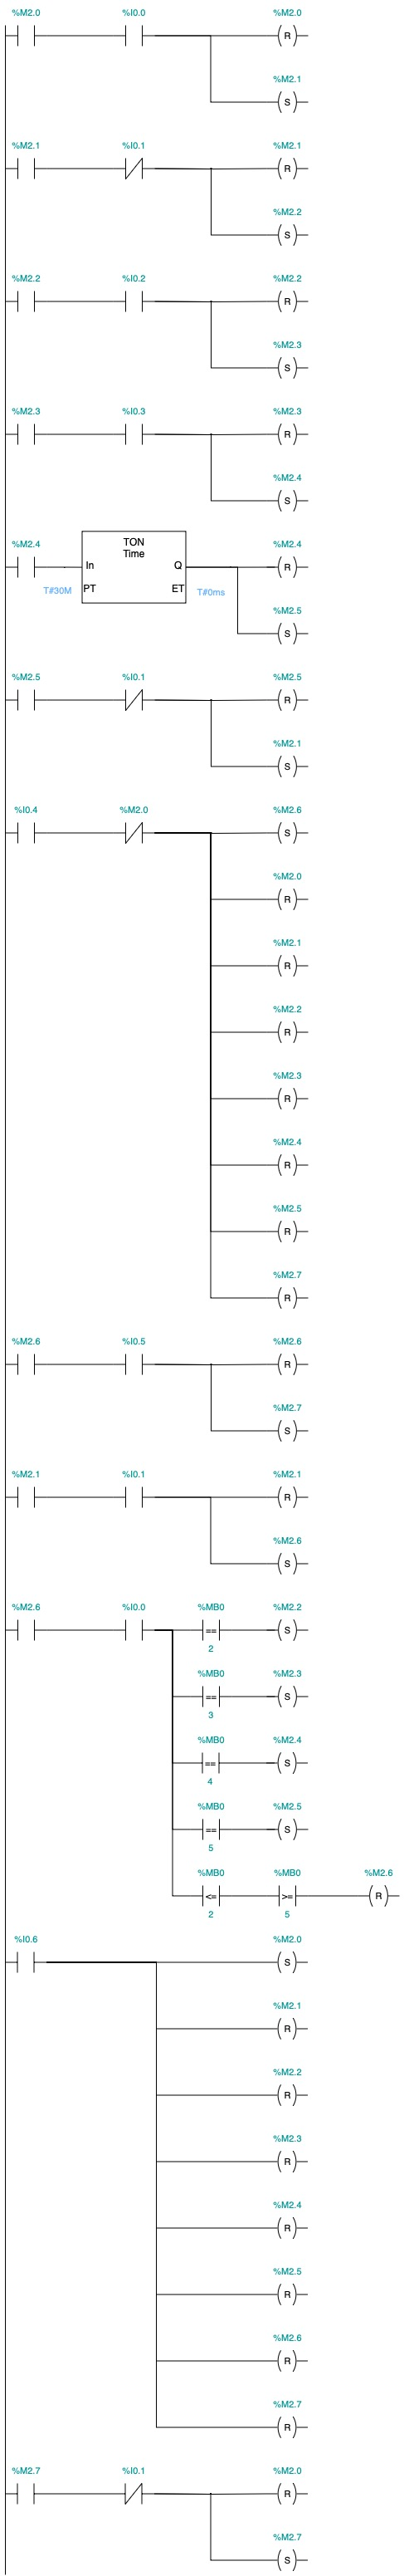
\includegraphics[trim={0 43cm 0 55cm}, clip, scale=.5]{img/Ladder_diagram_2.jpg}
    \caption{State Machine - Ladder diagram part 6}
    \label{fig:ladder26}
\end{figure}
\end{frame}

\begin{frame}
\frametitle{Ladder Diagram}
\framesubtitle{State Machine}
\begin{figure}
    \centering
    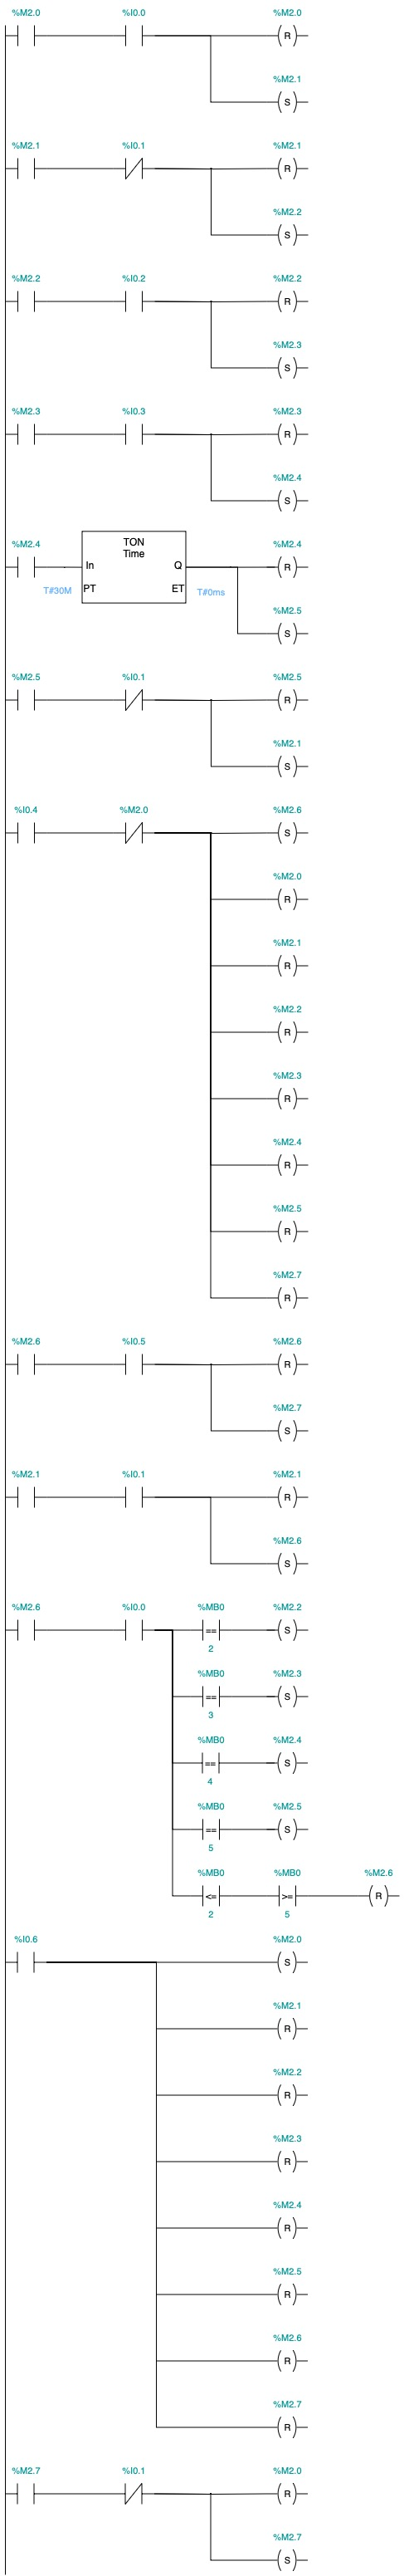
\includegraphics[trim={0 32cm 0 66cm}, clip, scale=.5]{img/Ladder_diagram_2.jpg}
    \caption{State Machine - Ladder diagram part 7}
    \label{fig:ladder27}
\end{figure}
\end{frame}

\begin{frame}
\frametitle{Ladder Diagram}
\framesubtitle{State Machine}
\begin{figure}
    \centering
    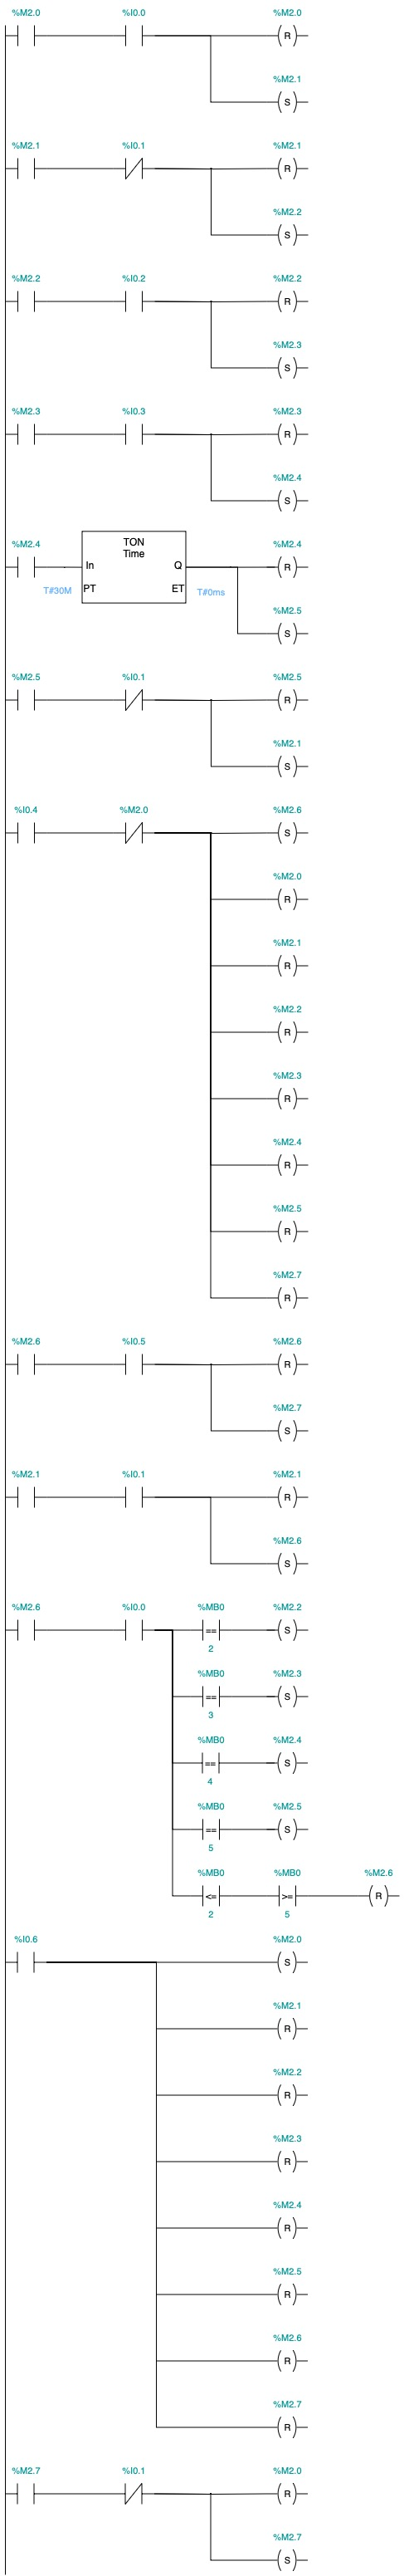
\includegraphics[trim={0 21cm 0 77cm}, clip, scale=.5]{img/Ladder_diagram_2.jpg}
    \caption{State Machine - Ladder diagram part 8}
    \label{fig:ladder28}
\end{figure}
\end{frame}

\begin{frame}
\frametitle{Ladder Diagram}
\framesubtitle{State Machine}
\begin{figure}
    \centering
    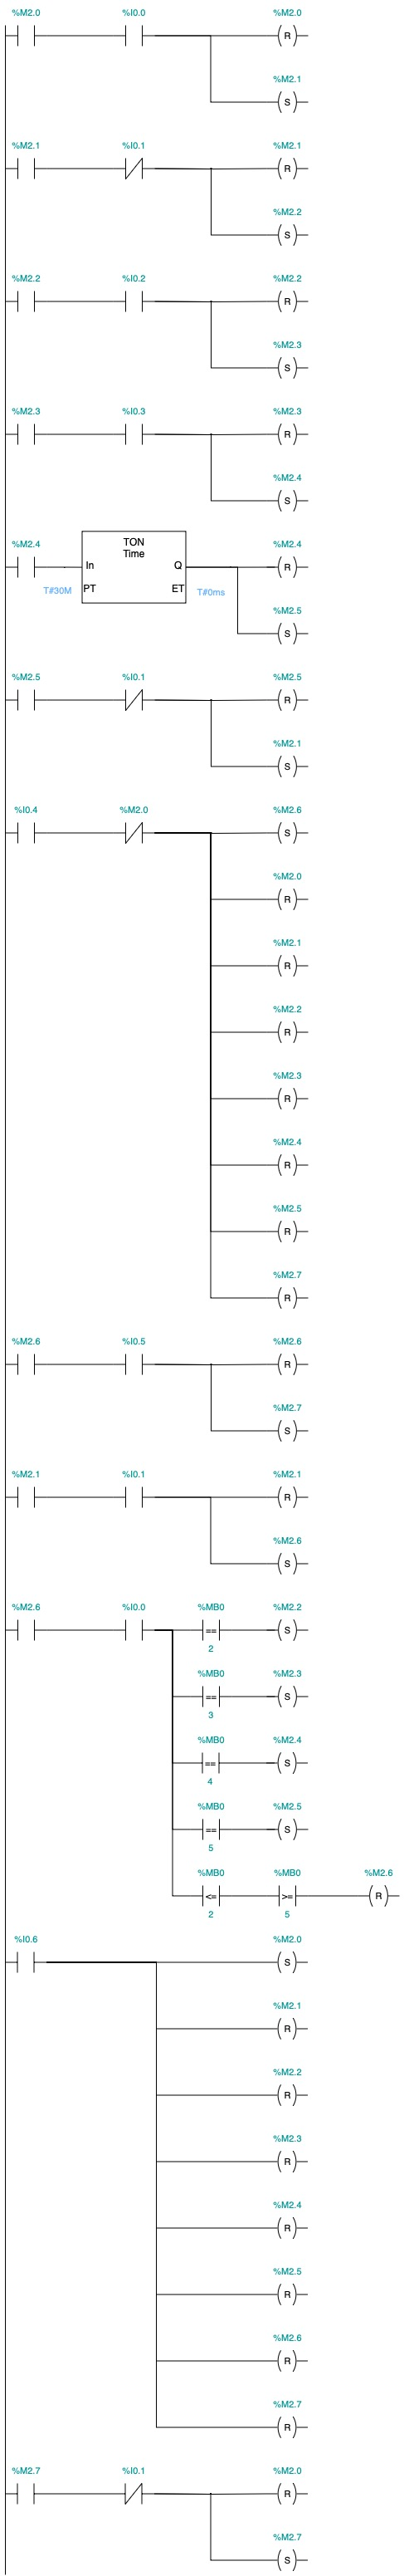
\includegraphics[trim={0 10cm 0 88cm}, clip, scale=.5]{img/Ladder_diagram_2.jpg}
    \caption{State Machine - Ladder diagram part 9}
    \label{fig:ladder29}
\end{figure}
\end{frame}

\begin{frame}
\frametitle{Ladder Diagram}
\framesubtitle{State Machine}
\begin{figure}
    \centering
    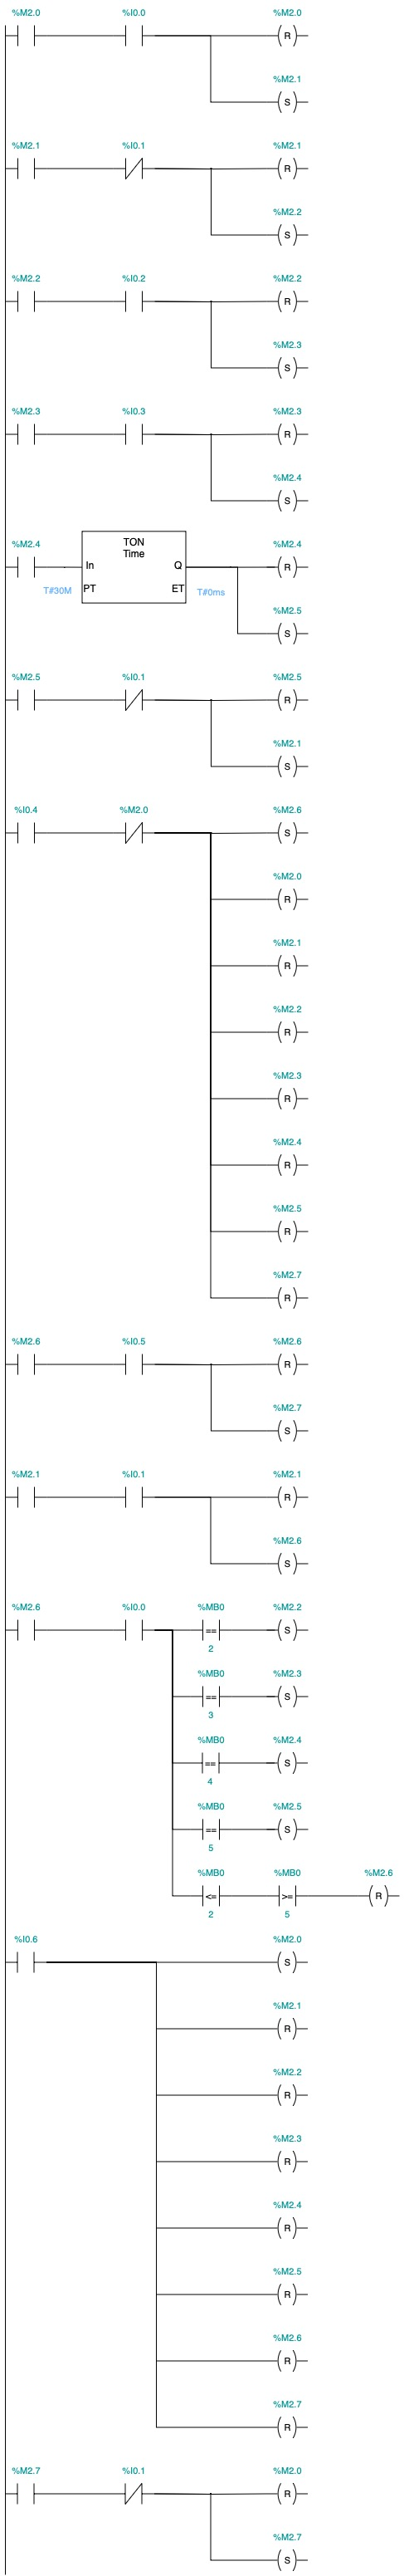
\includegraphics[trim={0 0 0 99cm}, clip, scale=.5]{img/Ladder_diagram_2.jpg}
    \caption{State Machine - Ladder diagram part 10}
    \label{fig:ladder210}
\end{figure}
\end{frame}

\begin{frame}
\frametitle{Ladder Diagram}
\framesubtitle{}
\begin{figure}
    \centering
    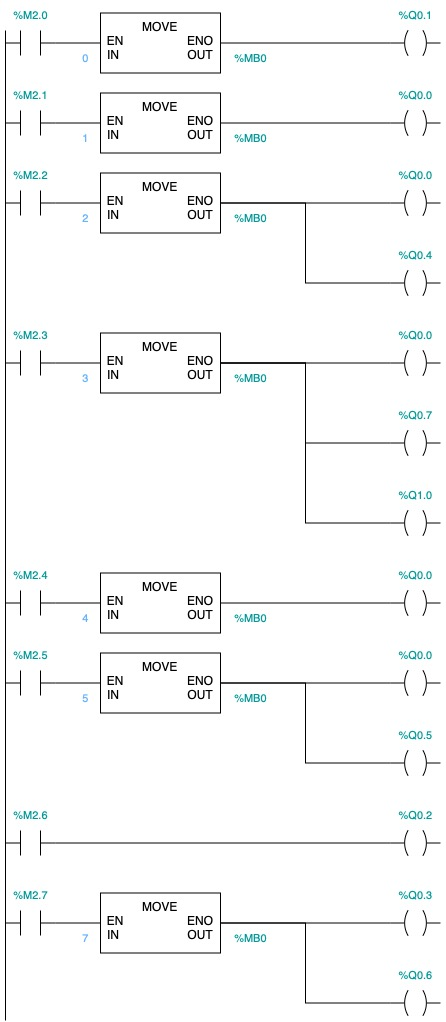
\includegraphics[trim={0 25cm 0 0}, clip, scale=.5]{img/Ladder_diagram_3.jpg}
    \caption{Busines Logic - Ladder diagram part 1}
    \label{fig:ladder31}
\end{figure}
\end{frame}

\begin{frame}
\frametitle{Ladder Diagram}
\framesubtitle{}
\begin{figure}
    \centering
    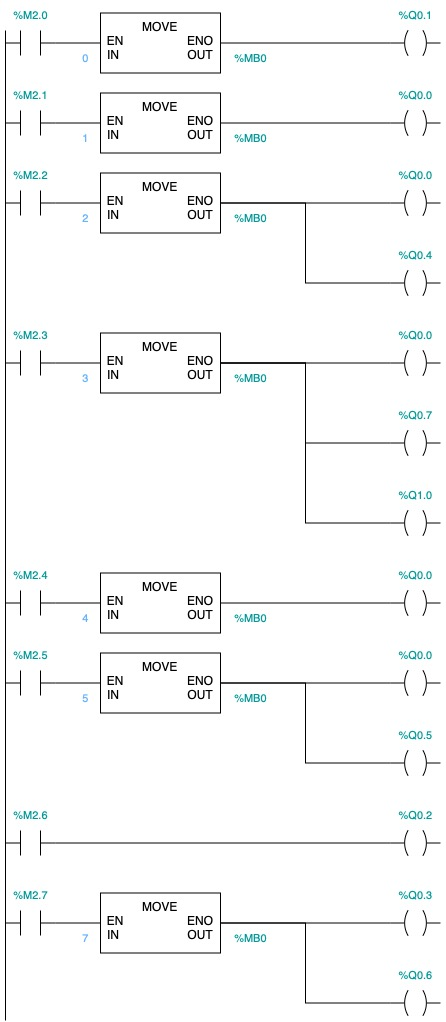
\includegraphics[trim={0 13cm 0 11cm}, clip, scale=.5]{img/Ladder_diagram_3.jpg}
    \caption{Busines Logic - Ladder diagram part 2}
    \label{fig:ladder32}
\end{figure}
\end{frame}

\begin{frame}
\frametitle{Ladder Diagram}
\framesubtitle{}
\begin{figure}
    \centering
    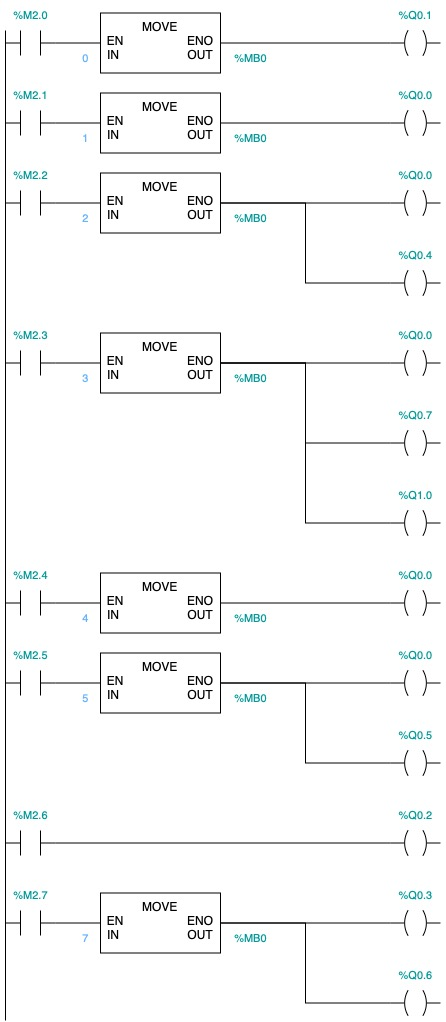
\includegraphics[trim={0 0cm 0 23cm}, clip, scale=.5]{img/Ladder_diagram_3.jpg}
    \caption{Busines Logic - Ladder diagram part 3}
    \label{fig:ladder33}
\end{figure}
\end{frame}

\begin{frame}
\frametitle{Components Choice}
\framesubtitle{}
\begin{itemize}
    \item \textbf{Water level sensors:} FST700-204 Modbus Capacitive Liquid Electronic Oil Level Sensor 198.54\$ x2 $\approx$ 361.70€
    \item \textbf{Residual chlorine sensor:} Sensorex FCL502-MA 1293.88€
    \item \textbf{Industrial tank mixer:} Savino Barbera AN30 direct-drive mixer
    \item \textbf{Water pumps:} Savino Barbera OP125E horizontal pump
    \item \textbf{Chlorine pump:} Savino Barbera OA20 horizontal pump
\end{itemize}
\end{frame}

\end{document}